\documentclass[12pt]{article}
\usepackage[letterpaper]{geometry}
\usepackage[parfill]{parskip}
\usepackage{setspace}
\doublespacing
\usepackage{enumitem}
\usepackage{graphicx}
\usepackage{amssymb}
\usepackage{amsmath}
\usepackage{mathtools}
\usepackage{mathrsfs}
\usepackage{epstopdf}
\usepackage{pdflscape}
\usepackage{float}
\usepackage{breqn}
\usepackage{cancel}
\usepackage[short]{optidef}
\usepackage[style=authoryear, backend=biber]{biblatex}
\addbibresource{jessoe_rapson_notes_bibliography.bib}

\newcommand{\diff}{\mathop{}\!\mathrm{d}}
\newcommand{\Lagr}{\mathcal{L}}

\title{Notes for Jessoe and Rapson}
\author{Churn Ken Lee}
\date{}   
\begin{document}
\maketitle

\section{Summary}
\begin{itemize}
    \item RCT study of the effect of price changes on electricity usage
    \item 2 treatment groups:
        \begin{itemize}
            \item price increase
            \item price increase + in-house display (IHD)
        \end{itemize}
    \item Both groups decrease usage, but price+IHD group is more elastic
\end{itemize}

\section{Background}
\begin{itemize}
    \item Households' electricity demand is inelastic (\cite{reiss_white_2005}; \cite{alcott_2011}; \cite{ito_2014})
    \item Could be due to lack of full information; price vs non-price attributes:
        \begin{itemize}
            \item Price salience
                \begin{itemize}
                    \item Taxes on price tags (\cite{chetty_looney_kroft_2009})
                    \item eBay shipping and handling fees (\cite{hossain_morgan_2006})
                    \item Electronic toll collection (\cite{finkelstein_2009})
                \end{itemize}
            \item Non-price attributes 
                \begin{itemize}
                    \item household consumption of services, not direct inputs, e.g., durables that convert inputs into outputs
                \end{itemize}
        \end{itemize}
    \item Quantity of electricity consumed hidden due to infrequent billing
    \item Households could be inelastic, or just appear to be inelastic due to lack of complete information
\end{itemize}

\section{Experimental details}
\subsection{Context}
\begin{itemize}
    \item Partnership with United Illuminating Company (UI), a regulated electric utility in Connecticut
    \item Field experiment in Bridgeport and New Haven, July and August 2011
    \item Short-term price increases and real-time information
\end{itemize}

\subsection{Experimental setup}
\begin{itemize}
    \item Eligibility: live in townhouse or single family home, broadband Inernet, sign agreement
    \item Incentive: \$20 for completion of pre-survey prior to assignment, \$20 for completion of survey after end of pilot
    \item Recruitment: 60,000 emails to customers with paperless billing, 1,152 participants
    \item Sample: 437 households
    \item Randomly assigned into 3 groups:
        \begin{itemize}
            \item Control: 207 households
            \item Price-only: 130 households exposed to pricing events
            \item Price+IHD: 100 households esposed to pricing events, but also receive real-time information via in-home displays (IHD)
        \end{itemize}
    \item IHD removes information acquisition cost as it provides real-time usage, electricity price, estimated monthly usage and bill-to-date
    \item
    \resizebox{1\linewidth}{!}{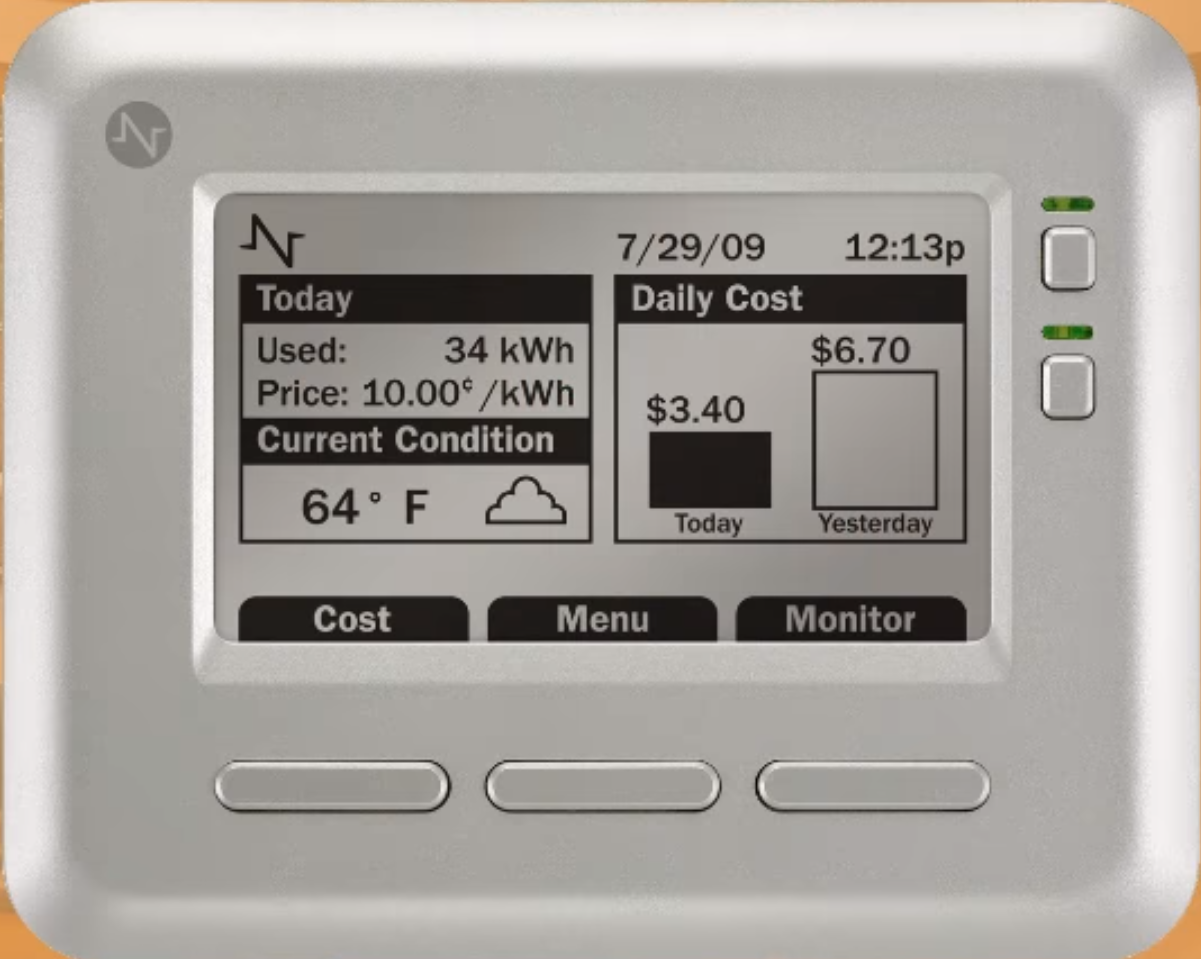
\includegraphics{ihd1.png}}
    \resizebox{1\linewidth}{!}{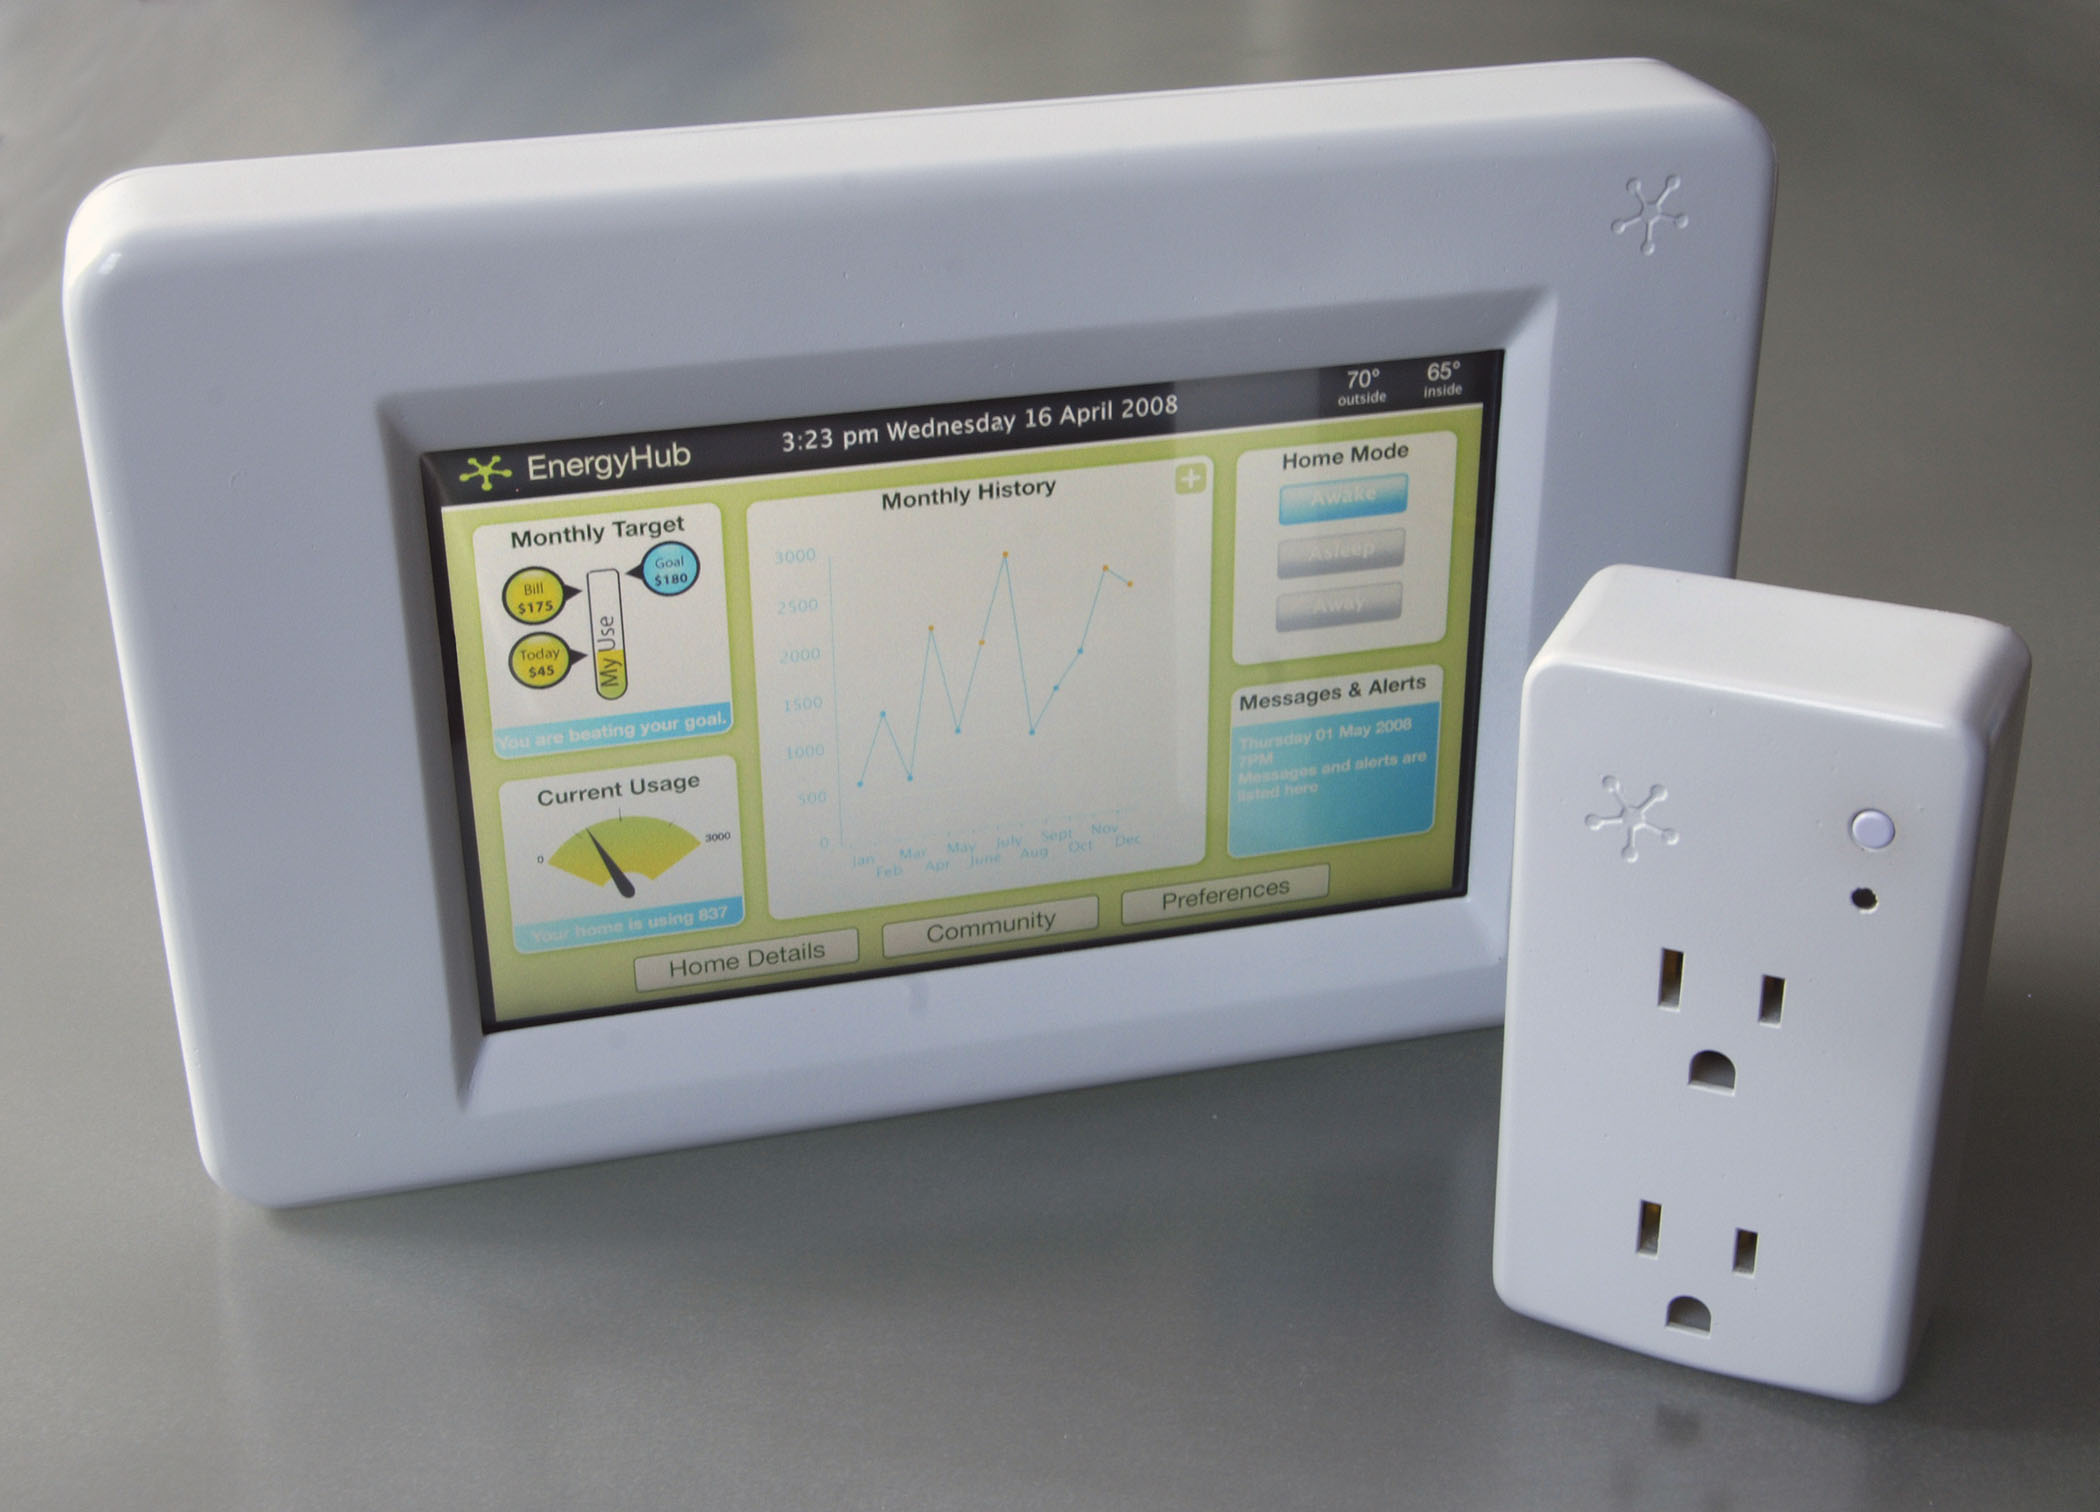
\includegraphics{ihd2.jpg}}
    \item Allows households to learn about electrical consumption by appliance, enabling better optimization
    \item 2 types of pricing events:
        \begin{itemize}
            \item Day ahead (DA): notification one day prior of a \$0.50 increase in per-kWh price of electricity (250\% increase on base price of \$0.20 per-kWh)
            \item Thity minutes (TM): notification 30 minutes before a \$1.25 increase in per-kWh price of electricity (625\% increase on base price)
        \end{itemize}
    \item \resizebox{1\linewidth}{!}{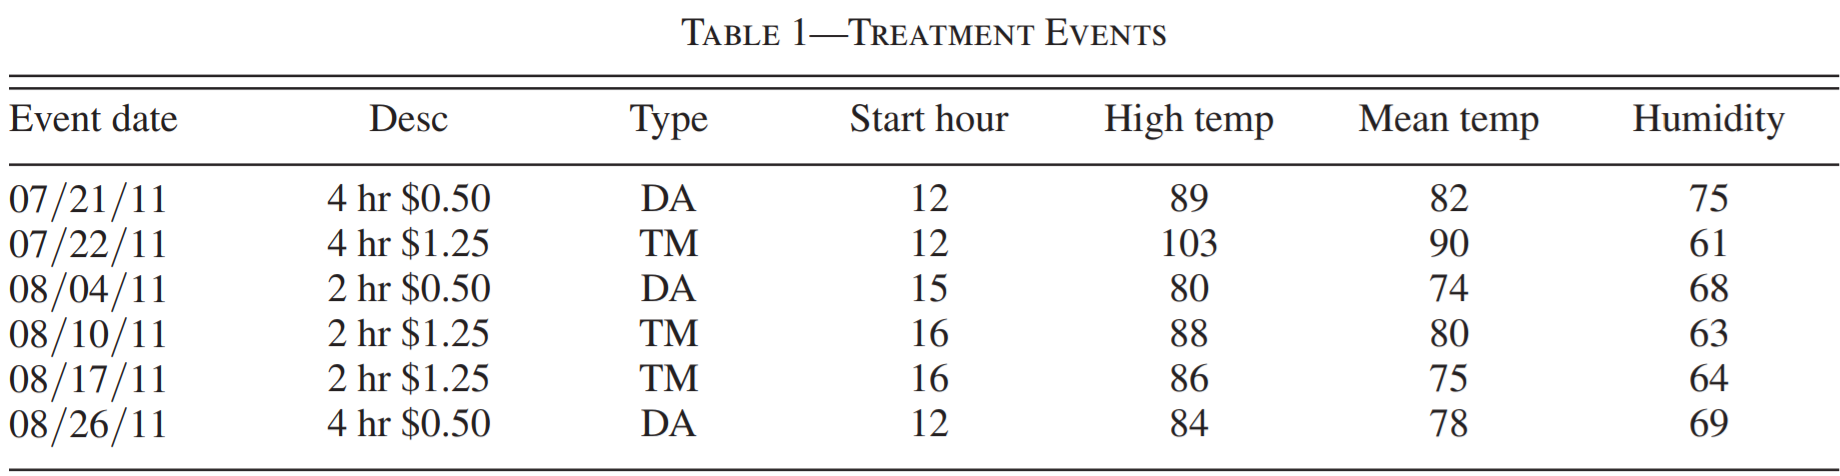
\includegraphics{pricing_events.png}}
    \item Notification received via phone-call, email, or text messages
    \item Transmission of incentives via off-bill account credited with \$100
    \item (Amount of electricity consumed during pricing event)$*$(increase in price during pricing event) is subtracted from off-bill account, and remaining amount given to customer
\end{itemize}

\section{Data}
\begin{itemize}
    \item High-frequency meter data on household electricity usage, collected in 15-minute intervals
    \item Data on receipt of event notification
    \item 2 surveys: demographics, housing unit characteristics, appliance ownership, conservation-related actions, tendency to be home during the day, frequency of use of IHD
    \item Technical software issue: random missing observations
    \item Balance seems good
    \item \resizebox{1\linewidth}{!}{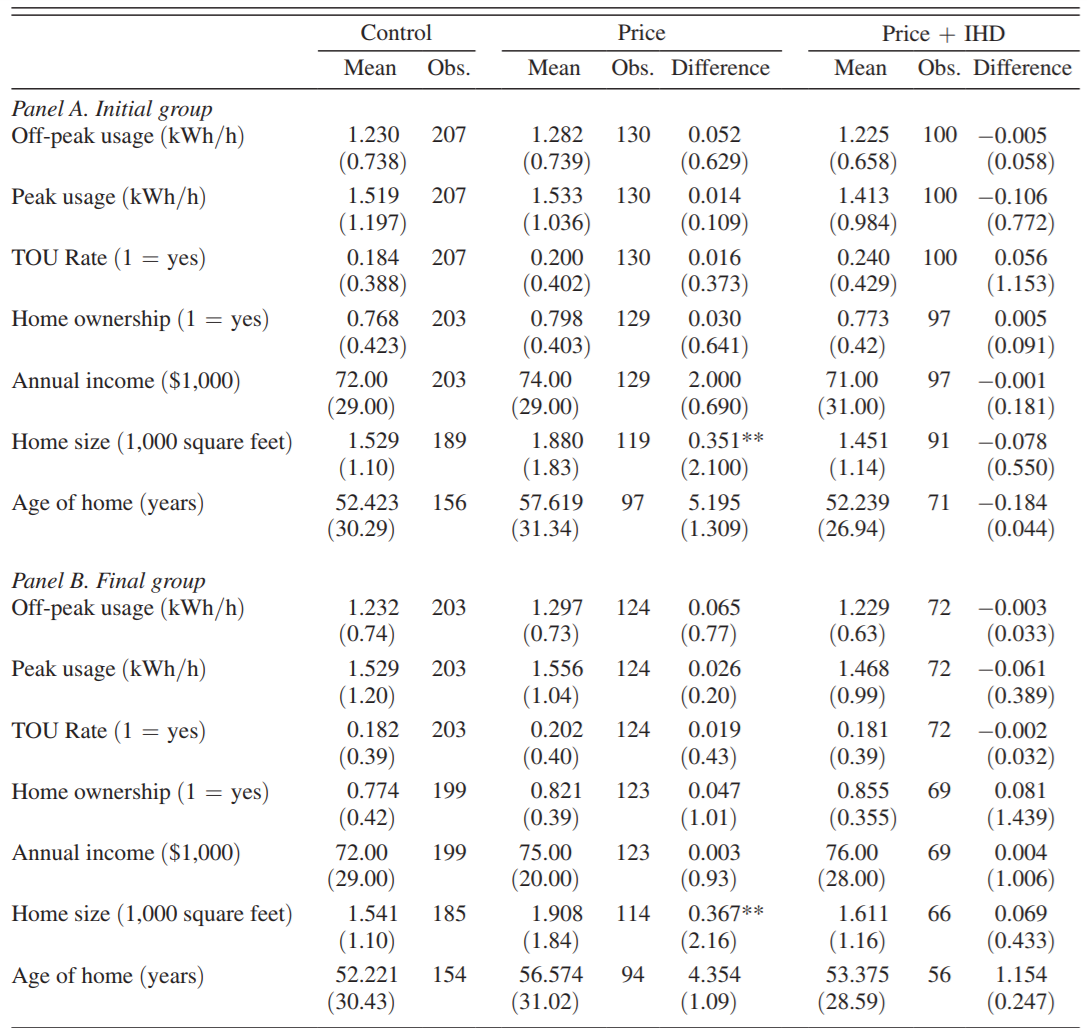
\includegraphics{balance.png}}
    \item Attriton: 38 households did not complete: 4 control, 6 price-only, 28 price+IHD
    \item Estimate LPM of treatment indicator on mean off-peak usage and rate class; neither variable is significant
    \item Estimate LPM of compliance dummy on mean off-peak usage and rate class; rate class is significant, suggesting selective attrition
    \item \resizebox{1\linewidth}{!}{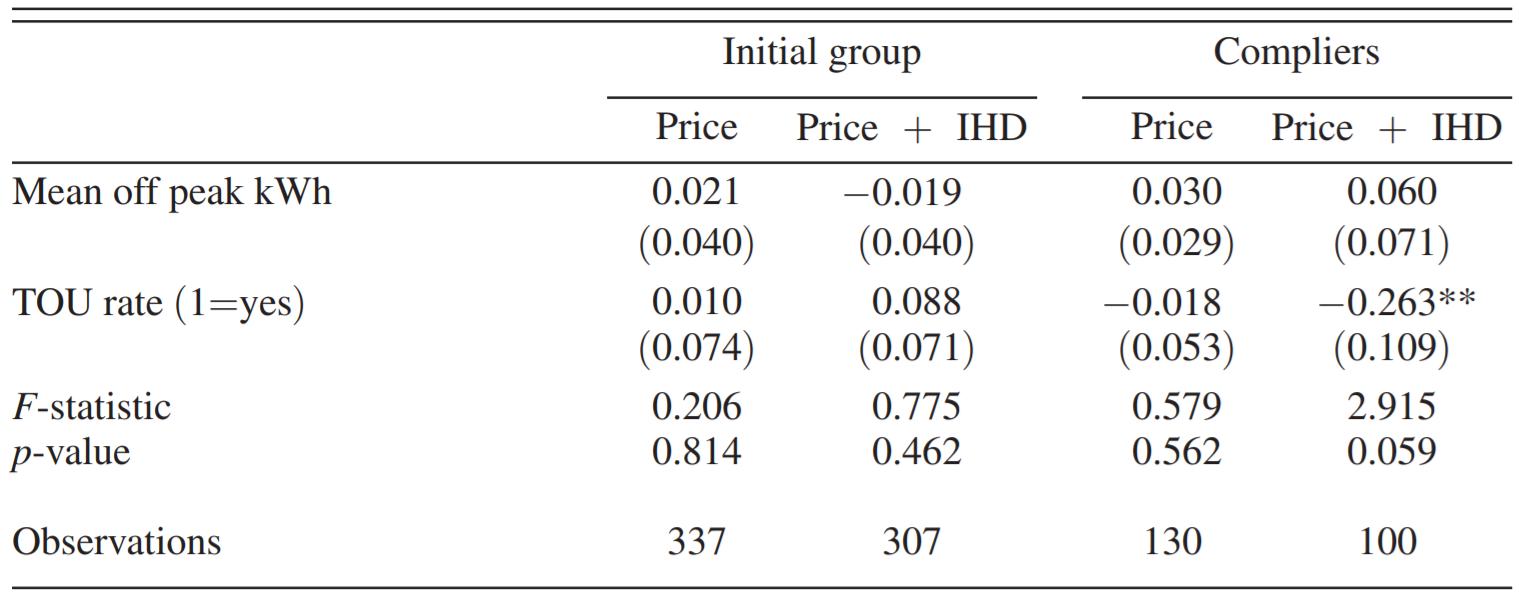
\includegraphics{lpm.png}}
\end{itemize}

\section{Raw data and mean difference}
\begin{itemize}
    \item Price+IHD group consume less during pricing events relative to other groups
    \item \resizebox{1\linewidth}{!}{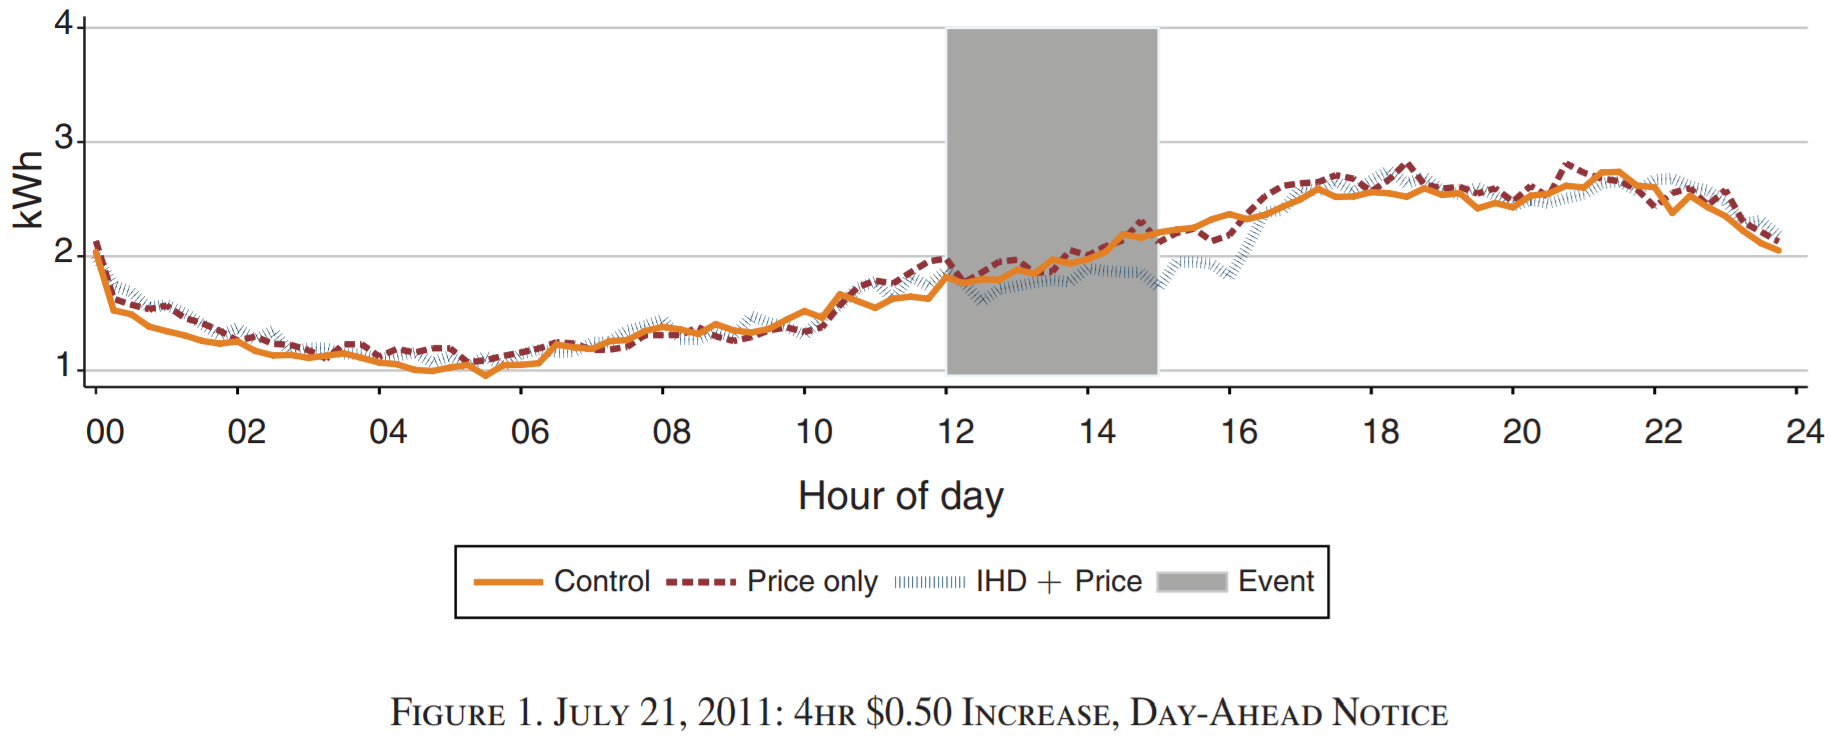
\includegraphics{raw1.png}}
    \item \resizebox{1\linewidth}{!}{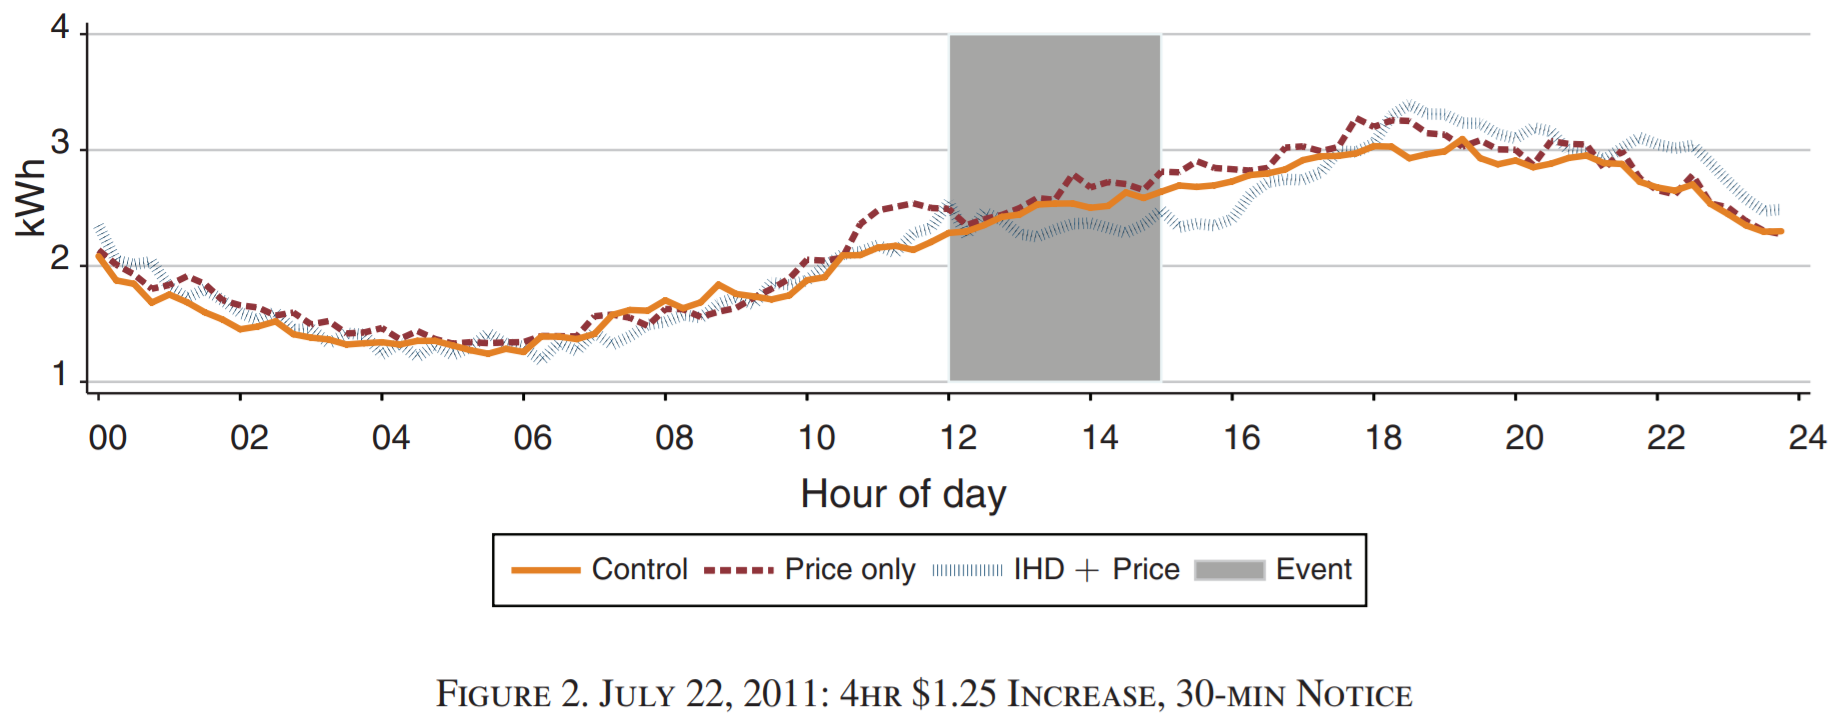
\includegraphics{raw2.png}}
    \item \resizebox{1\linewidth}{!}{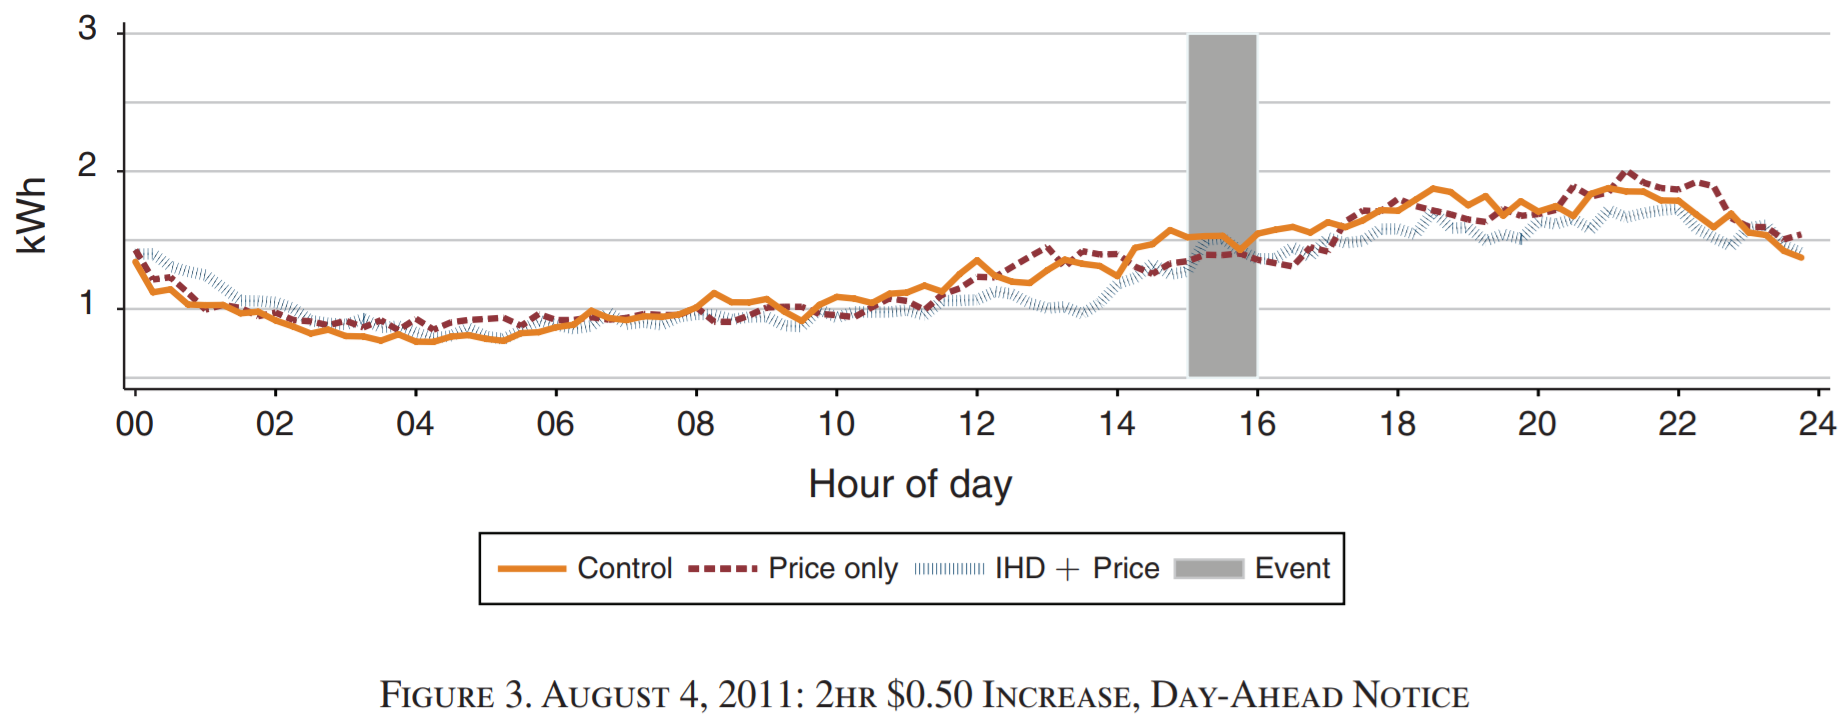
\includegraphics{raw3.png}}
    \item \resizebox{1\linewidth}{!}{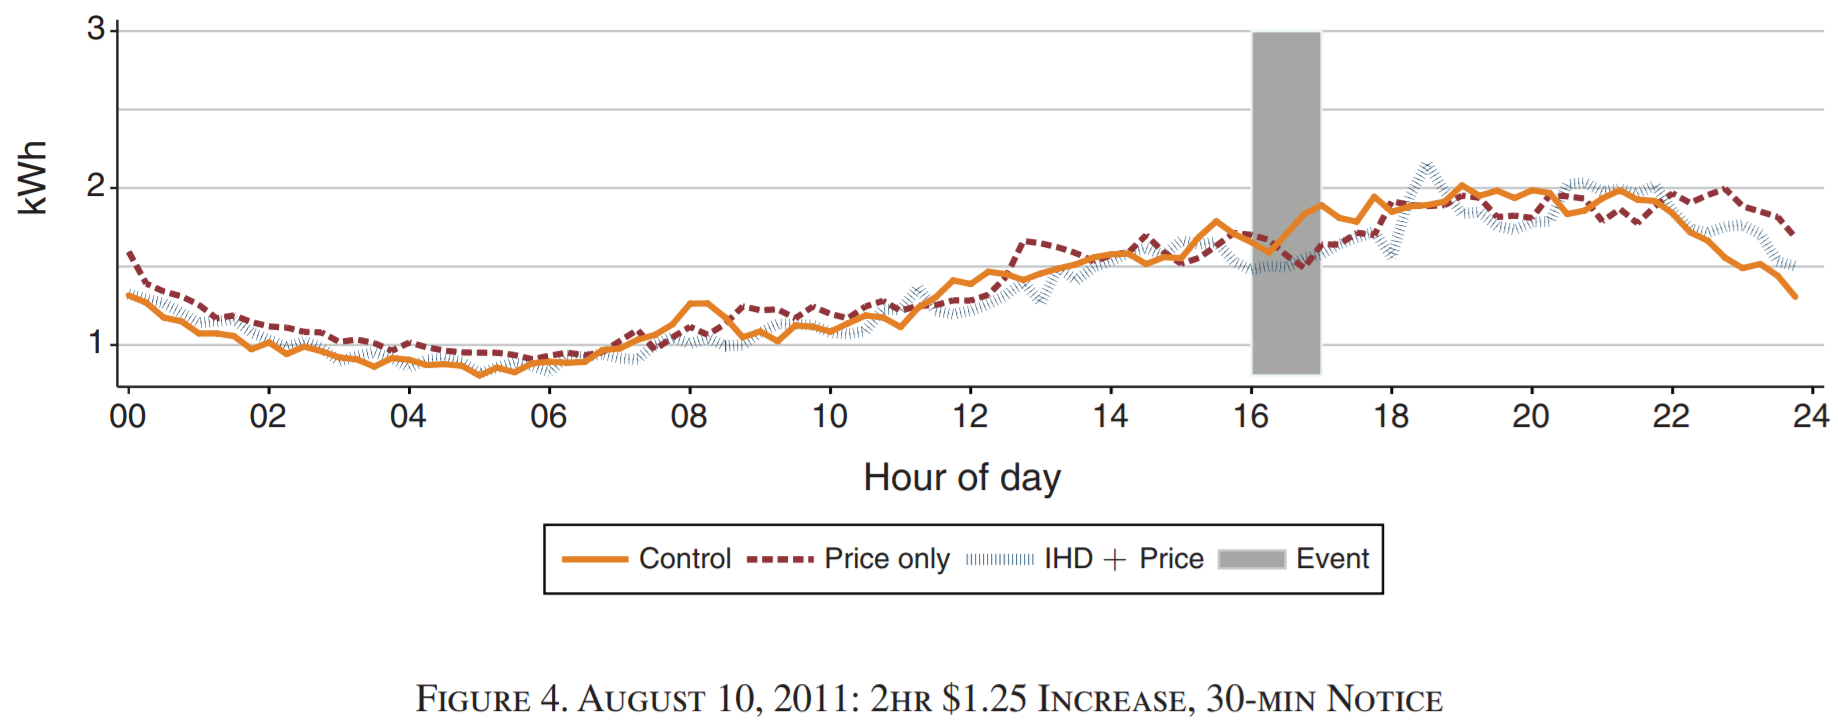
\includegraphics{raw4.png}}
    \item \resizebox{1\linewidth}{!}{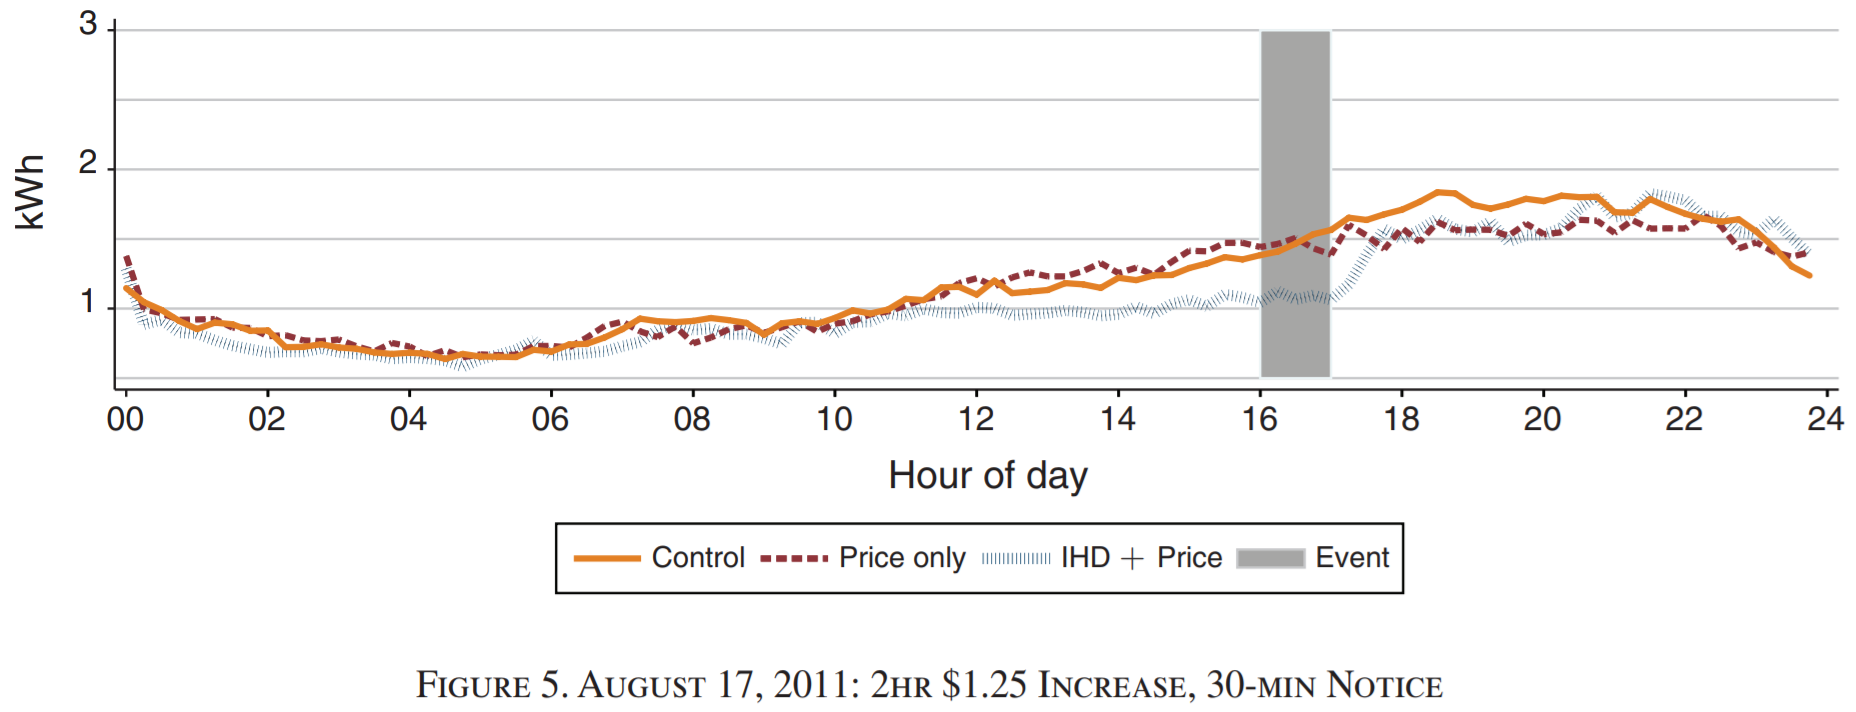
\includegraphics{raw5.png}}
    \item \resizebox{1\linewidth}{!}{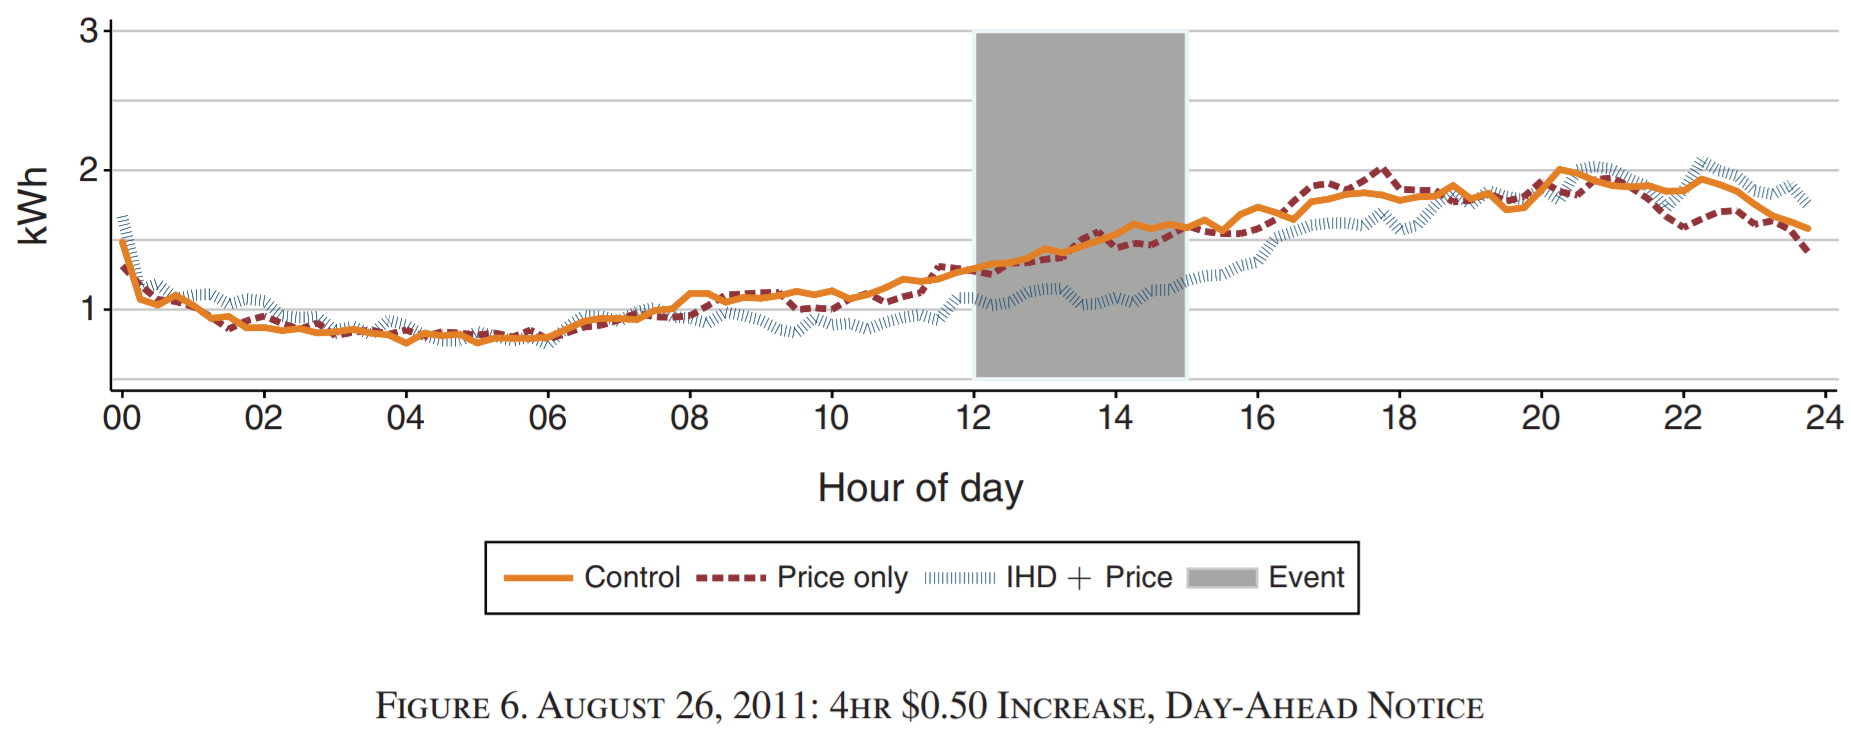
\includegraphics{raw6.png}}
    \item \resizebox{1\linewidth}{!}{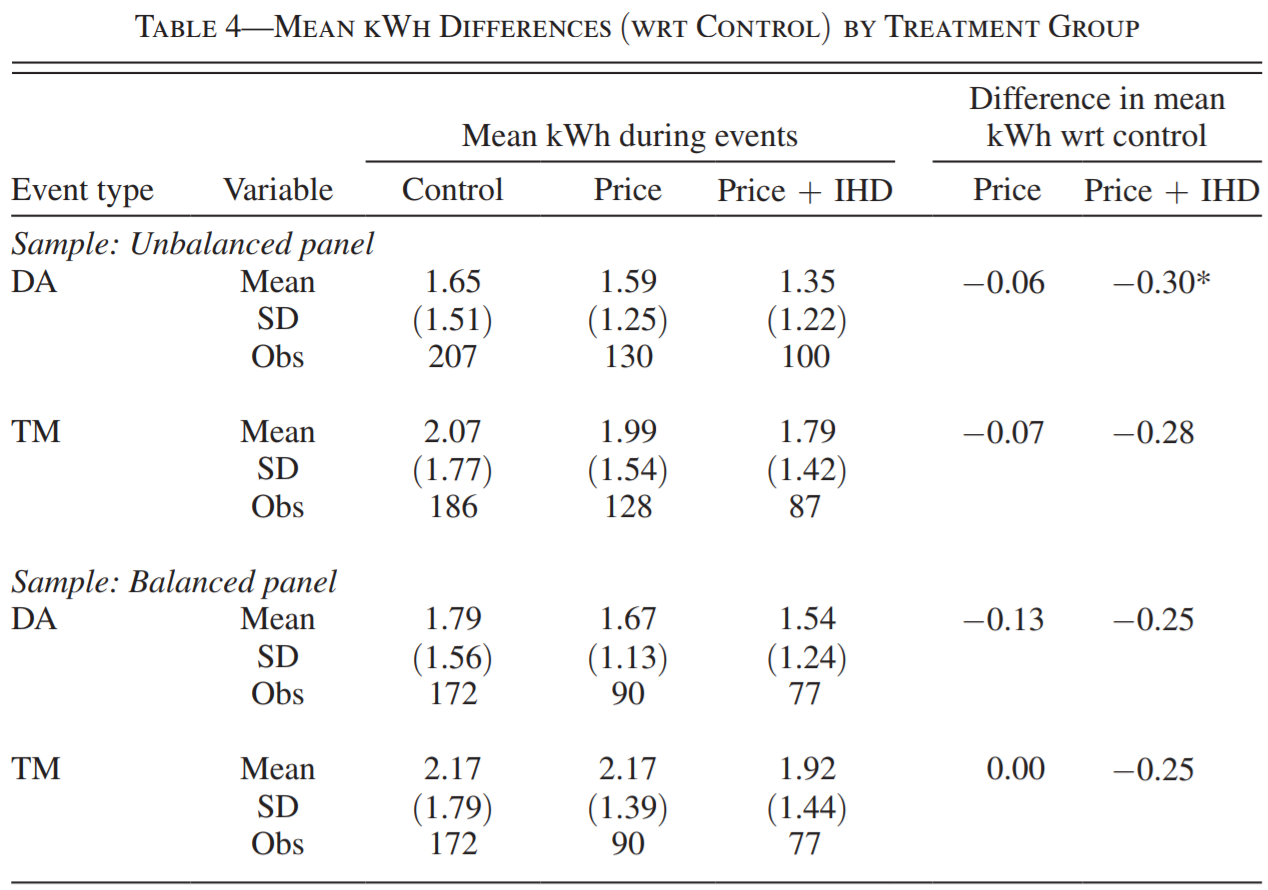
\includegraphics{diff_mean.png}}
\end{itemize}

\section{Results}
\subsection{Intent-to-treat (ITT)}
\begin{itemize}
    \item Simple DiD equation:
        \begin{align*}
            q _ { i t } = \sum _ { g \in \{ P , P + I \} } \beta _ { g } D _ { i t } ^ { g } + \gamma _ { g } + \delta _ { e } + \mu _ { i t }
        \end{align*}
    \item Also include hour-by-calendar-date dummies and household fixed effects
\end{itemize}

\subsection{Treatment effect on treated (TOT)}
\begin{itemize}
    \item Instrument for receipt of treatment using initial assignment
    \item Obtain slightly larger coefficients
    \item Arc elasticity: 0.12
    \item \resizebox{1\linewidth}{!}{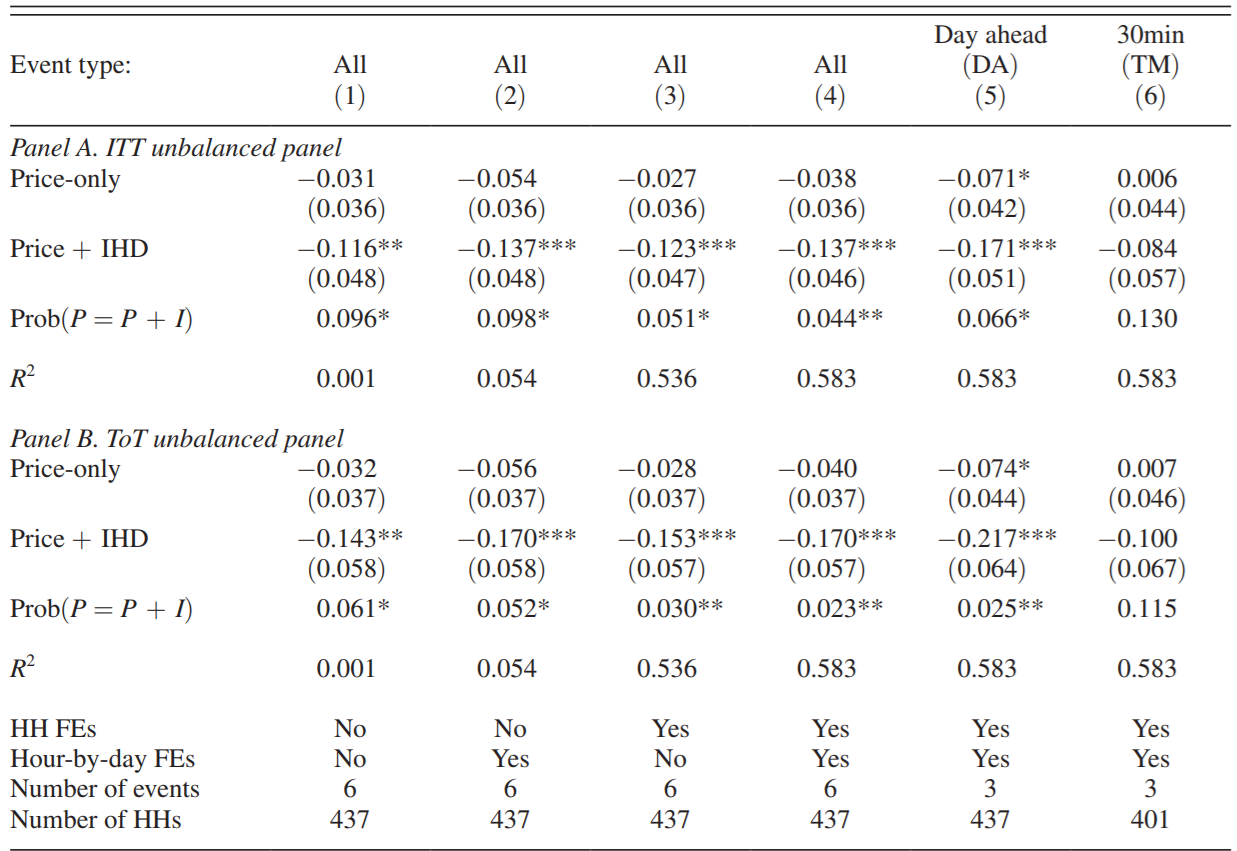
\includegraphics{results.png}}
\end{itemize}

\subsection{Price events or learning?}
\begin{itemize}
    \item 2 possible channels via IHD: increase awareness of price events and learning
    \item To eliminate price channel, add confirmation of receipt of notification variable, interact with treatment dummies
    \item Estimation equation is
        \begin{align*}
            q _ { i t } = \sum _ { g \in \{ P , P + I \} A \in \{ 0,1 \} } \beta _ { g } D _ { i t } ^ { g } \times 1 A _ { i t = A }  + \gamma _ { i } + \sigma _ { h } + \mu _ { i t }
        \end{align*}
    \item \resizebox{1\linewidth}{!}{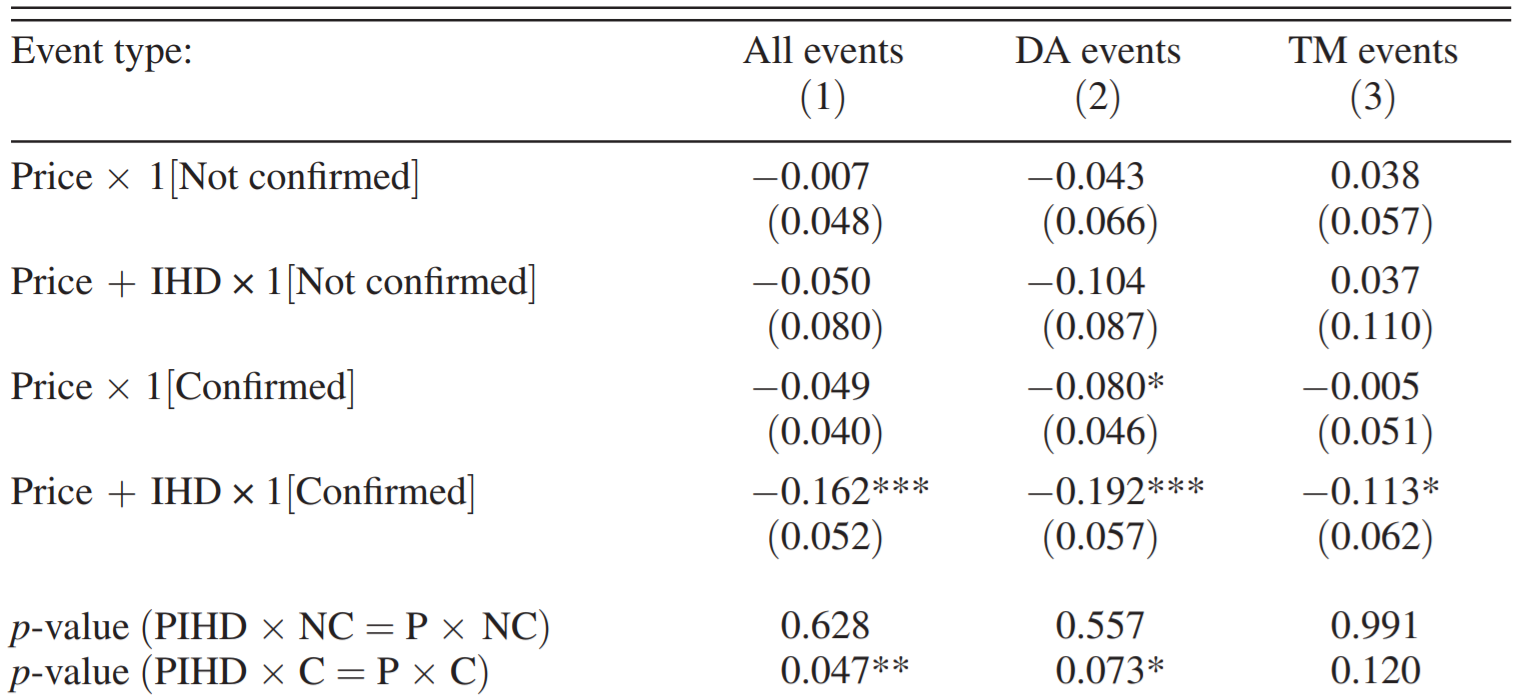
\includegraphics{confirmation.png}}
    \item Conditional on confirmation of receipt, statistically significant difference between price-only and price+IHD group
    \item Conditional on non-confirmation of receipt, no statistically significant difference between price-only and price+IHD group
    \item Evidence against price event awareness
    \item Now interact treatment dummy with indicator variables for frequency of IHD interaction
    \item \resizebox{1\linewidth}{!}{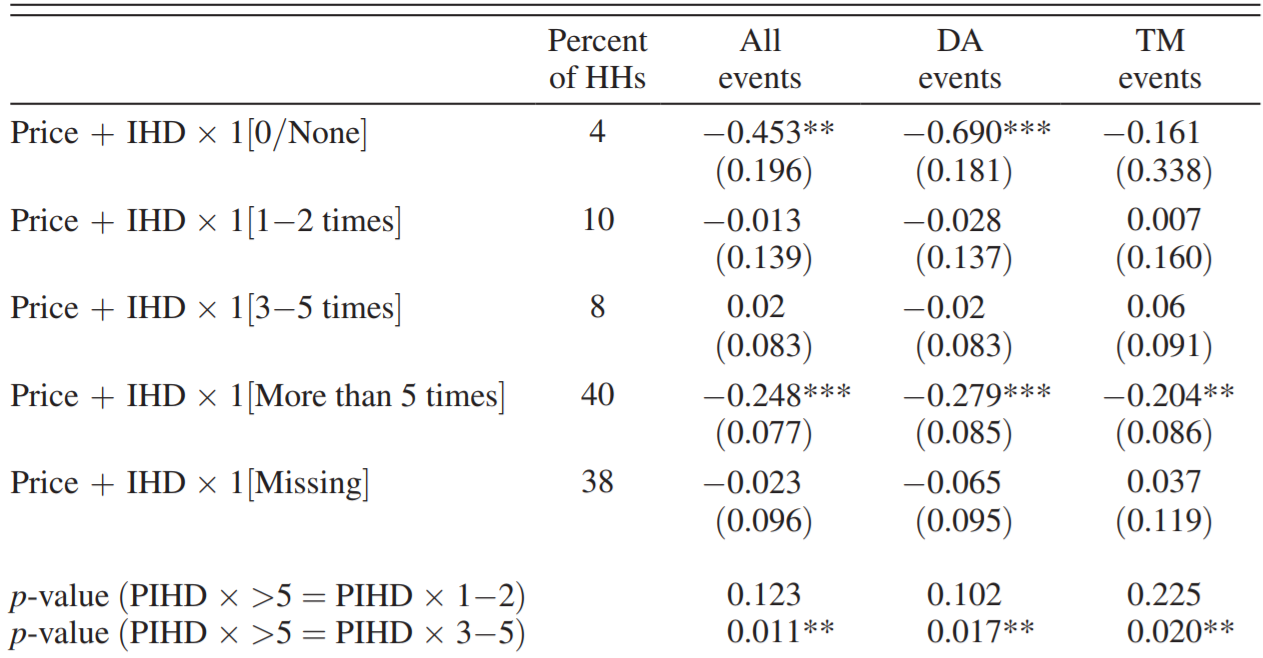
\includegraphics{ihd_freq.png}}
    \item Higher frequency $\Rightarrow$ larger response
    \item 
\end{itemize}

\section{Conservation}
\begin{itemize}
    \item Add indicator for periods 2 hours before and after price events
    \item Price+IHD has large decrease in these periods for DA events but price-only has no decrease for DA events
    \item Both price-only and price+IHD has no response for TM events
    \item \resizebox{1\linewidth}{!}{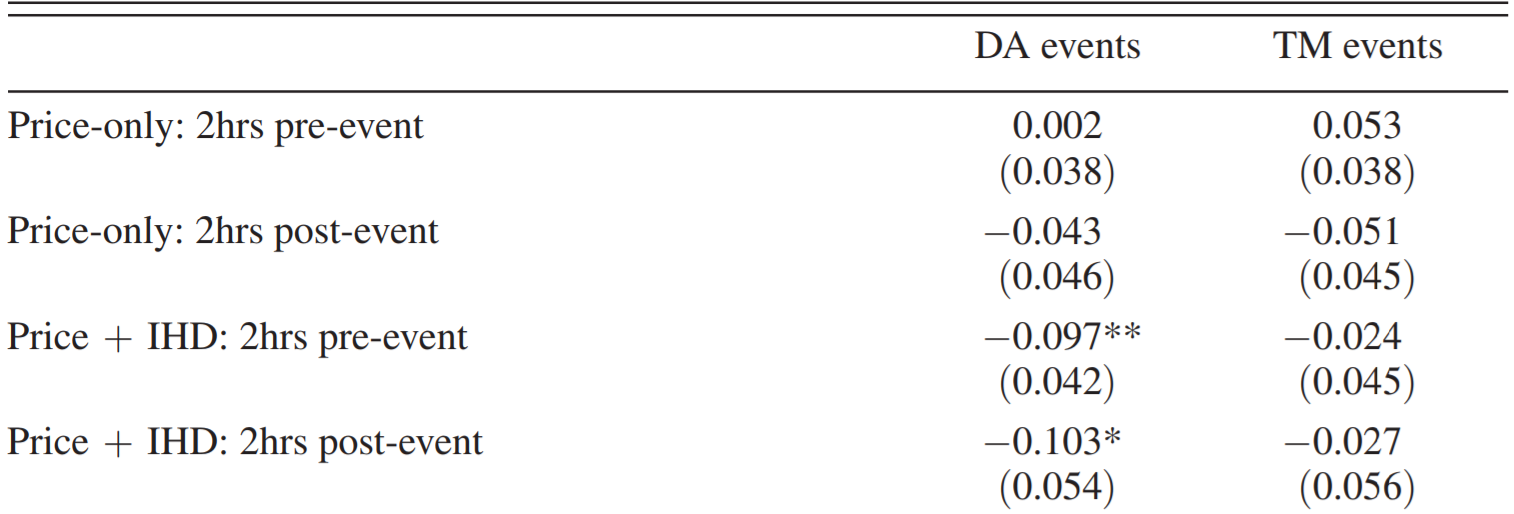
\includegraphics{prepost.png}}
    \item Evidence of habit formation: average daily decrease in usage for different times
        \begin{align*}
            q _ { i t } = \sum _ { g } \beta _ { g } D _ { i t } ^ { g } + \sum _ { g } \sum _ { h o d } \lambda _ { g , h o d } \times D _ { i } ^ { g } \times d + \gamma _ { i } + \sigma _ { h } + \mu _ { i t }
        \end{align*}
    \item \resizebox{1\linewidth}{!}{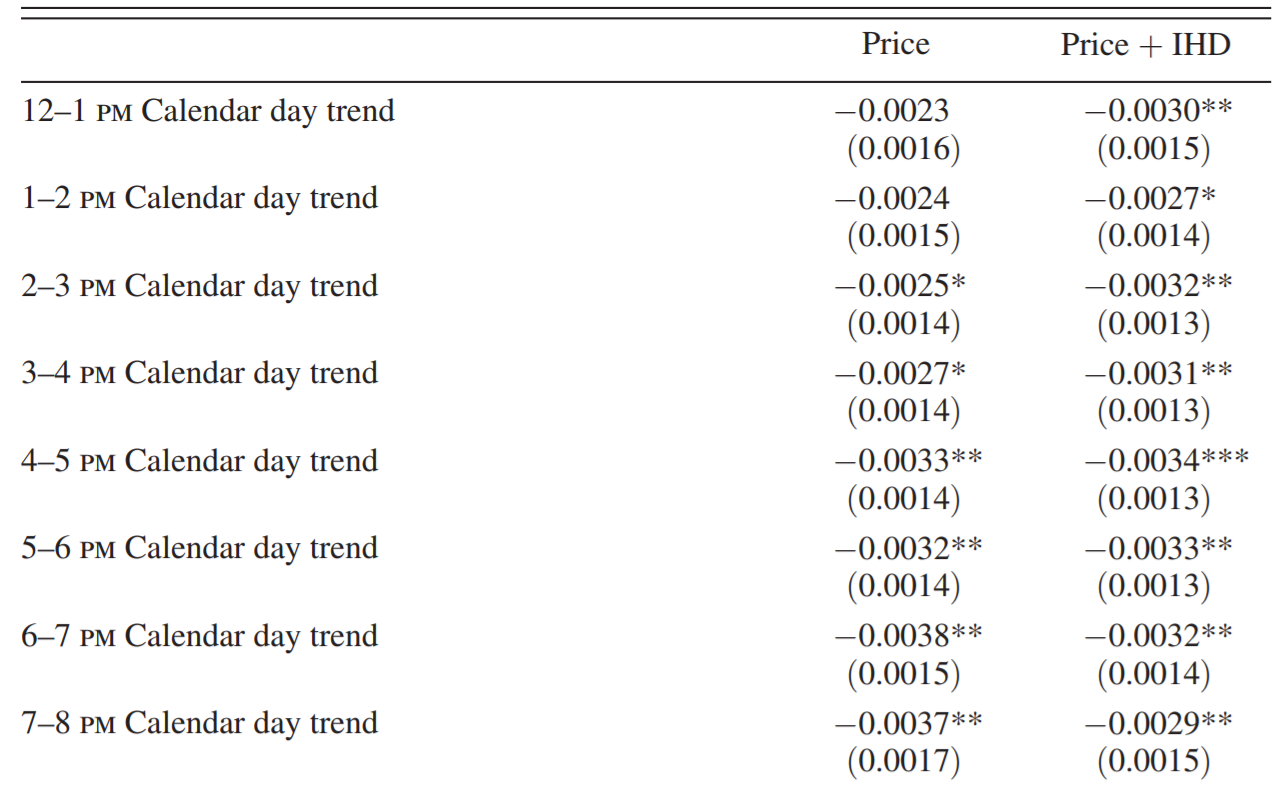
\includegraphics{habit.png}}
    \item Three observations
        \begin{itemize}
            \item Attenuation of main effect estimate: reduction in baseline usage to which event-period effects are compared. Also, spillovers larger for price+IHD group: even larger effect of information feedback on price elasticity
            \item Cumulative response similar irrespective of information feedback, but feedback may allow better response to short-run incentives
            \item Habit formation similar for both price-only and price+IHD groups, leading to large GHG abatement benefits
        \end{itemize}
\end{itemize}
\end{document}